% chapters/06-risk-management.tex

\chapter{Risk Management and Compliance}

\begin{importantbox}
This chapter provides a comprehensive framework for identifying, assessing, and mitigating risks in the Nigerian market, along with detailed compliance requirements by sector and region.
\end{importantbox}

\section{Due Diligence Framework}

\subsection{Core Due Diligence Components}

\begin{figure}[htbp]
    \centering
    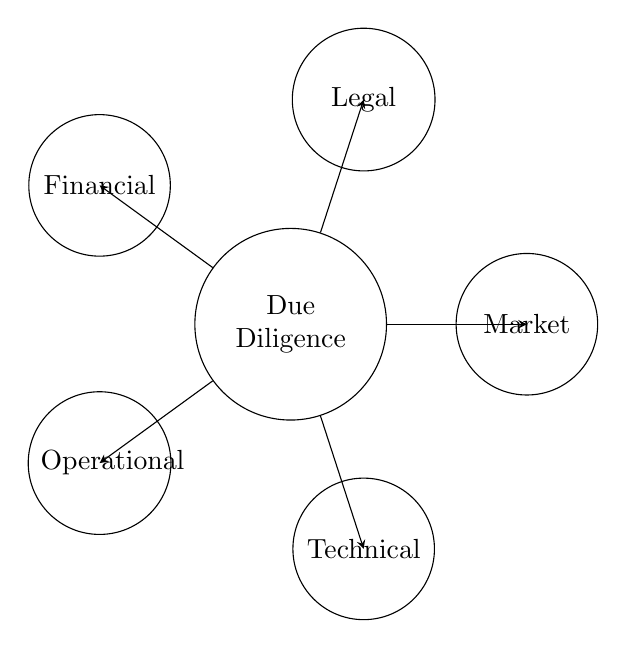
\begin{tikzpicture}[node distance=2cm]
        % Core node
        \node[draw, circle, text width=2cm, align=center] (core) {Due\\Diligence};

        % Surrounding nodes with better spacing
        \foreach \angle/\label in {
            0/Market,
            72/Legal,
            144/Financial,
            216/Operational,
            288/Technical
        } {
            \node[draw, circle, text width=1.5cm, align=center]
                at (\angle:3) {\label};
            \draw[-stealth] (core) -- (\angle:3);
        }
    \end{tikzpicture}
    \caption{Due Diligence Framework}
    \label{fig:due-diligence}
\end{figure}

\subsection{Risk Assessment Matrix}
\begin{center}
\begin{tabularx}{\textwidth}{>{\raggedright\arraybackslash}X >{\centering\arraybackslash}X >{\centering\arraybackslash}X >{\raggedright\arraybackslash}X}
    \toprule
    \textbf{Risk Type} & \textbf{Likelihood} & \textbf{Impact} & \textbf{Mitigation Strategy} \\
    \midrule
    Regulatory & High & High & Compliance partners \\
    Market & Medium & High & Phased entry \\
    Operational & Medium & Medium & Local expertise \\
    Financial & Medium & High & Risk management \\
    Technical & Low & Medium & Testing protocols \\
    \bottomrule
\end{tabularx}
\end{center}

\FloatBarrier
\section{Legal Safeguards}

\begin{warningbox}
Legal requirements can change frequently. Always verify current requirements through official channels or your legal counsel.
\end{warningbox}

\subsection{Essential Legal Documentation}
\begin{tcolorbox}[colback=white,colframe=primarydark,title=\textbf{Documentation Checklist}]
\begin{itemize}
    \item Registration certificates
    \item Operating licenses
    \item Tax registrations
    \item Regulatory permits
    \item Employment contracts
    \item Partnership agreements
\end{itemize}
\end{tcolorbox}

\FloatBarrier
\section{Regional Compliance Requirements}

\begin{regionalbox}{United Kingdom}
\textbf{Financial Services Compliance Framework}
\begin{itemize}
    \item FCA compliance requirements
    \item Anti-money laundering regulations
    \item Data protection standards
    \item Cross-border transaction rules
\end{itemize}
\end{regionalbox}

\FloatBarrier
\subsection{UK Compliance Timeline}
\begin{figure}[htbp]
    \centering
    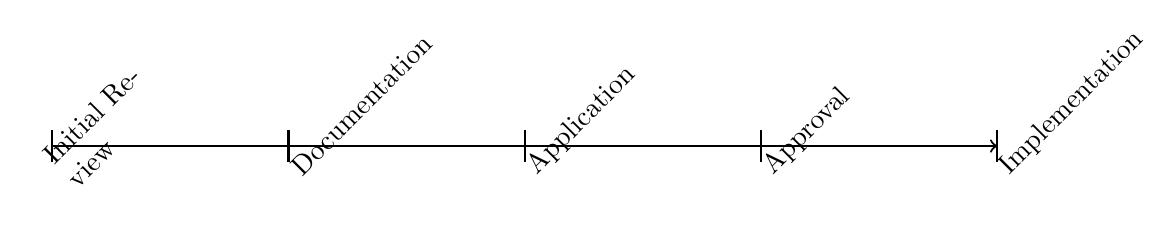
\begin{tikzpicture}
        % Timeline with better spacing and labels
        \draw[thick,->] (0,0) -- (12,0);
        \foreach \x/\label in {
            0/Initial Review,
            3/Documentation,
            6/Application,
            9/Approval,
            12/Implementation
        } {
            \draw[thick] (\x,0.2) -- (\x,-0.2);
            \node[text width=2cm, align=left, rotate=45, anchor=west]
                at (\x,-0.4) {\label};
        }
    \end{tikzpicture}
    \caption{UK Financial Services Compliance Process}
    \label{fig:uk-compliance}
\end{figure}

\begin{regionalbox}{United States}
\textbf{Tech Regulation and Data Protection}
\begin{itemize}
    \item Data privacy requirements
    \item IP protection framework
    \item Consumer protection standards
    \item Digital security compliance
\end{itemize}

\subsection{US Tech Compliance Matrix}
\begin{center}
\begin{tabularx}{\textwidth}{>{\raggedright\arraybackslash}X >{\centering\arraybackslash}X >{\raggedright\arraybackslash}X}
    \toprule
    \textbf{Requirement} & \textbf{Standard} & \textbf{Implementation} \\
    \midrule
    Data Privacy & GDPR-aligned & Privacy framework \\
    Security & ISO 27001 & Security protocols \\
    Consumer Protection & FTC standards & Protection measures \\
    \bottomrule
\end{tabularx}
\end{center}
\end{regionalbox}

\begin{regionalbox}{UAE}
\textbf{Trade Compliance Framework}
\begin{itemize}
    \item Trade license requirements
    \item Import/export regulations
    \item Customs documentation
    \item Currency controls
\end{itemize}

\subsection{UAE Trade Compliance Checklist}
\begin{tcolorbox}[colback=white,colframe=primary,title=\textbf{Required Documents}]
\begin{itemize}
    \item Trade license
    \item Chamber of Commerce registration
    \item Import/export permits
    \item Customs registration
    \item Bank references
\end{itemize}
\end{tcolorbox}
\end{regionalbox}

\begin{regionalbox}{Canada}
\textbf{Environmental and Agricultural Compliance}
\begin{itemize}
    \item Environmental standards
    \item Agricultural regulations
    \item Food safety requirements
    \item Export compliance
\end{itemize}

\subsection{Canadian Sector Compliance}
\begin{center}
\begin{tabularx}{\textwidth}{>{\raggedright\arraybackslash}X >{\centering\arraybackslash}X >{\raggedright\arraybackslash}X}
    \toprule
    \textbf{Sector} & \textbf{Standards} & \textbf{Certifications} \\
    \midrule
    Agriculture & CFIA standards & Safety certificates \\
    Environment & ISO 14001 & Environmental permits \\
    Food Processing & HACCP & Safety certifications \\
    \bottomrule
\end{tabularx}
\end{center}
\end{regionalbox}

\FloatBarrier
\section{Banking and Money Transfer}

\subsection{Banking Structure}
\begin{figure}[htbp]
    \centering
    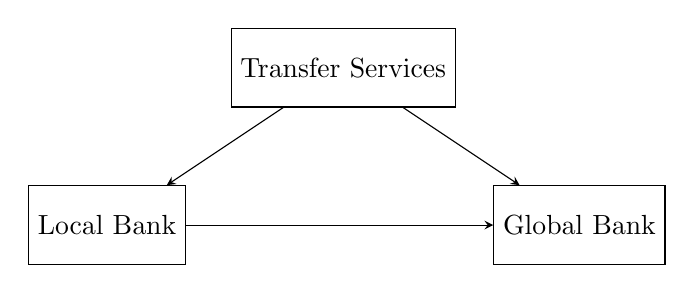
\begin{tikzpicture}[
        node distance=2cm,
        box/.style={draw, minimum width=2cm, minimum height=1cm}
    ]
        % Banking structure diagram with improved spacing
        \node[box] (local) at (0,0) {Local Bank};
        \node[box] (global) at (6,0) {Global Bank};
        \node[box] (transfer) at (3,2) {Transfer Services};
        \draw[-stealth] (local) -- (global);
        \draw[-stealth] (transfer) -- (local);
        \draw[-stealth] (transfer) -- (global);
    \end{tikzpicture}
    \caption{Cross-Border Banking Structure}
    \label{fig:banking-structure}
\end{figure}

\FloatBarrier
\section{Currency Risk Management}

\begin{tcolorbox}[colback=white,colframe=primarydark,title=\textbf{Currency Risk Mitigation Strategies}]
\begin{itemize}
    \item Forward contracts
    \item Currency hedging
    \item Local currency accounts
    \item Payment timing strategies
\end{itemize}
\end{tcolorbox}

\begin{communitybox}
Access additional risk management resources on the Africa Growth Circle:
\begin{itemize}
    \item Risk assessment templates
    \item Compliance checklists
    \item Expert advisory sessions
    \item Regulatory updates
    \item Due diligence guides
\end{itemize}
Visit circle.counseal.com for risk management support.
\end{communitybox}

% End of chapter workshop
\begin{workshopbox}
\textbf{Chapter 6 Risk Management Workshop}

1. Risk Assessment
\begin{itemize}
    \item Key risks identified: \_\_\_\_\_\_\_\_\_
    \item Risk priority ranking: \_\_\_\_\_\_\_\_\_
    \item Mitigation strategies: \_\_\_\_\_\_\_\_\_
\end{itemize}

2. Compliance Planning
\begin{itemize}
    \item Required permits: \_\_\_\_\_\_\_\_\_
    \item Documentation needed: \_\_\_\_\_\_\_\_\_
    \item Timeline for completion: \_\_\_\_\_\_\_\_\_
\end{itemize}

3. Banking Structure
\begin{itemize}
    \item Banking partners: \_\_\_\_\_\_\_\_\_
    \item Transfer mechanisms: \_\_\_\_\_\_\_\_\_
    \item Currency management: \_\_\_\_\_\_\_\_\_
\end{itemize}

Download comprehensive risk assessment templates from the Africa Growth Circle platform.
\end{workshopbox}

\begin{importantbox}
In Chapter 7, we'll explore building your local network and establishing key partnerships to help manage risks and ensure compliance.
\end{importantbox}